\chapter{图像的去噪方法}
\label{chap:Denoising}

图像去噪的目的是从噪声图像中恢复出干净的图像,这是低级视觉任务中的一个经典问题。由于干净的图像通常是未知的,因此这个问题本质上是不适当的。换句话说,它是一个欠定的映射问题,其中图像变换不是唯一的。一般来说,残差图像$ F $可以表示为$ F = yf(x)$,其中$ x $是噪声图像,$ f $是映射函数,它接收输入图像并将其转换为输出图像。 $ y $是理想的清洁图像。通过适应不同类型的映射函数,相同的数学模型适用于大多数其他低级别成像问题,如图像去模糊,去马赛克和超分辨率。

最近,深度神经网络在计算机视觉领域表现出了卓越的性能,从高级到低级任务。众所周知,神经网络能够将任何可测量的函数逼近到期望的准确度\cite{Hornik1989}。在图像去噪设置中,回归框架中的神经网络试图在某些输入噪声分布下逼近潜在条件期望值。当以监督方式训练前馈神经网络时,一个关键因素是选择损失函数来测量输出和地面真实图像之间的差异。最广泛使用的是每像素损失,其通过失真和参考图像像素的强度差异以及相关的峰值信噪比\cite{Wang2004}来计算。但是,每像素损失不能捕捉到感知差异,并且众所周知与感知图像质量的关联性很差\cite{Zhao2015,Zhanga2012}。这是因为当使用每像素丢失时隐含地做出的许多假设不被满足。可以说,最重要的是独立于图像的局部特征来处理噪声;相反,人类视觉系统(HVS)对噪声的敏感性取决于局部亮度,对比度和结构\citep{Wang2004}。

基于纯粹的学习策略,为图像去噪设计的一组深度神经网络已被证明优于其他被广泛接受的方法作为最先进的\cite{Burger2012}。但是,所有这些工作都存在一个问题:如果输入无噪音,则学习模型也会降低干净的图像质量。所以他们唯一的工作就是在他们接受训练的给定噪音水平下工作。用于噪声消除的标准通用算法应该能够处理不同级别的噪声,这种限制似乎需要一系列这样的网络,每个噪声级别一个。这是不切实际的,甚至是不现实的。因为我们不知道噪声水平和真实图像的类型。

我们的主要贡献简要概述如下:

\begin{enumerate}

\item 我们提出了一个非常深的全卷积体系结构,用于图像残差去噪。针对图像变换对残差映射函数进行建模,直接学习噪声分布。. 

\item 结合每像素和感知丢失函数的优点,训练具有低和高级别信息的转换网络,生成高质量的去噪图像。

\item 为使单个神经网络适用于所有噪声级别,我们研究网络的统计规律:使输入从不同噪声级别添加随机样本,输入也可以是干净的图像,因为学习的图像函数必须对干净的图像进行身份验证,训练有素的网络可以自动处理不同的级别。

\item 我们试验了一些常见的基准图像。结果表明我们的网络的优点和所提出的新型损失层克服了其他最近的图像去噪方面的最新技术方法。

\end{enumerate}

\section{相关工作}
已经提出了许多用于图像去噪的方法。一些有选择地平滑噪声图像的部分,目的是在保留图像细节的同时“平滑”噪声。一些方法将图像信号传送到可以容易地从信号中分离噪声的替代域。最近的方法利用图像的“非本地”统计:相同图像中的不同补丁在外观上通常相似。块匹配和3D过滤(BM3D)算法\cite{DBLP:journals/tip/DabovFKE07}通过协作过滤在变换域中对非局部相似补丁进行分组。 BM3D已经成为图像去噪的基准。

虽然BM3D是一种设计良好的算法,但基于学习的方法已经广泛用于图像去噪。神经网络方法和其他方法最显着的区别在于,它们通常自动直接从干净而嘈杂的图像中自动学习图像转换,而不是依赖人类先验。最近,由于深度神经网络的快速发展,许多新型的神经网络已经应用于图像去噪问题,如堆叠式稀疏自动编码器\cite{DBLP:conf/icml/VincentLBM08,DBLP:conf/nips/XieXC12,Agostinelli2013,Technologii2013a,Skribtsov2016},多层感知器\cite{Burger2012,Wang2014a},卷积网络\cite{Jain2009,Wu2014,Zhao2015,Mao2016,Eigen2013,Wu2014relu,Wang2015g}。

叠加去噪自动编码器\cite{DBLP:conf/icml/VincentLBM08}建立了使用去噪标准作为无监督目标的价值,以指导有用的更高级别表示的学习。去噪性能可以很容易地测量和直接优化。但是这种方法的目标是分类。 Xie等人提出了一种替代的监督训练方案 - 叠加稀疏降噪自动编码器(SSDA),该方法将稀疏编码和深度网络结合起来,用去噪自动编码器(DA)进行预训练,成功地将DA最初设计用于无监督特征学习,适用于图像去噪和盲目修补的任务。

Burger等\cite{Burger2012}提出了一种基于斑块的算法,该算法在具有普通多层感知器的大型数据集上学习,其性能优于BM3D。然而,他们的方法适合于单一级别的噪音,并且不能很好地推广到其他噪音级别。 Jain等人\cite{Jain2009}提出了深度卷积神经网络和无监督学习过程,该过程综合了特定噪声模型的训练样本。他们发现卷积网络在小波和马尔科夫随机场(MRF)方法中提供了可比较的并且在某些情况下更好的性能。

到目前为止,通过训练具有每像素损失函数的深度神经网络,已经解决了所有用于图像去噪任务的神经网络。但是在图像处理的情况下,这可能会受到特别的限制,因为每像素丢失与感知图像质量的相关性很低\cite{Zhao2015}。一些最近的论文已经使用优化来生成目标是感知的图像,这取决于从卷积网络提取的高级特征\cite{Dosovitskiy2016}。 \cite{Johnson2016,Mao2016}的工作与我们的工作特别相关,因为他们训练前馈神经网络以进行图像转换,他们使用预先训练用于图像分类的损失网络来定义感知损失函数,以测量输出的感知差异和地面实况。不过,他们专注于风格转换和图像超解像。后来的工作提出了编码器和解码器图像细节的卷积和解卷积层,并且使用对称跳跃连接来加速训练。但是图像的噪声只能通过卷积来捕获,并通过解卷积来恢复图像细节。我们的网络可以看作是具有对称跳转连接的整个转换函数。

Zhao等人\cite{Zhao2015}研究了包括感知驱动损失在内的多种损失的表现,并提出了一种新颖的可微分误差函数。从感知动机指标设计出一些新的损失层,它仍然专注于低级像素结构。
Wang等人的另一项工作\cite{Wang2014a}也与我们的研究特别相关,他们研究了自然图像斑块在线性变换方面的分布不变性,他们展示了如何使一个现有的深度神经网络在整个各级高斯噪声。然而,与上述方法不同,本文通过训练具有感知损失函数的前馈变换网络,将图像变换任务和基于优化的图像变换方法的优点相结合。同时通过显式训练不同级别的噪声并使原始图像作为输入,使单个深度神经网络在不同级别的加性高斯白噪声下工作良好。
\section{提出方法} 

\label{sec:method}
\begin{figure*}
\vspace{-6mm}
\centering
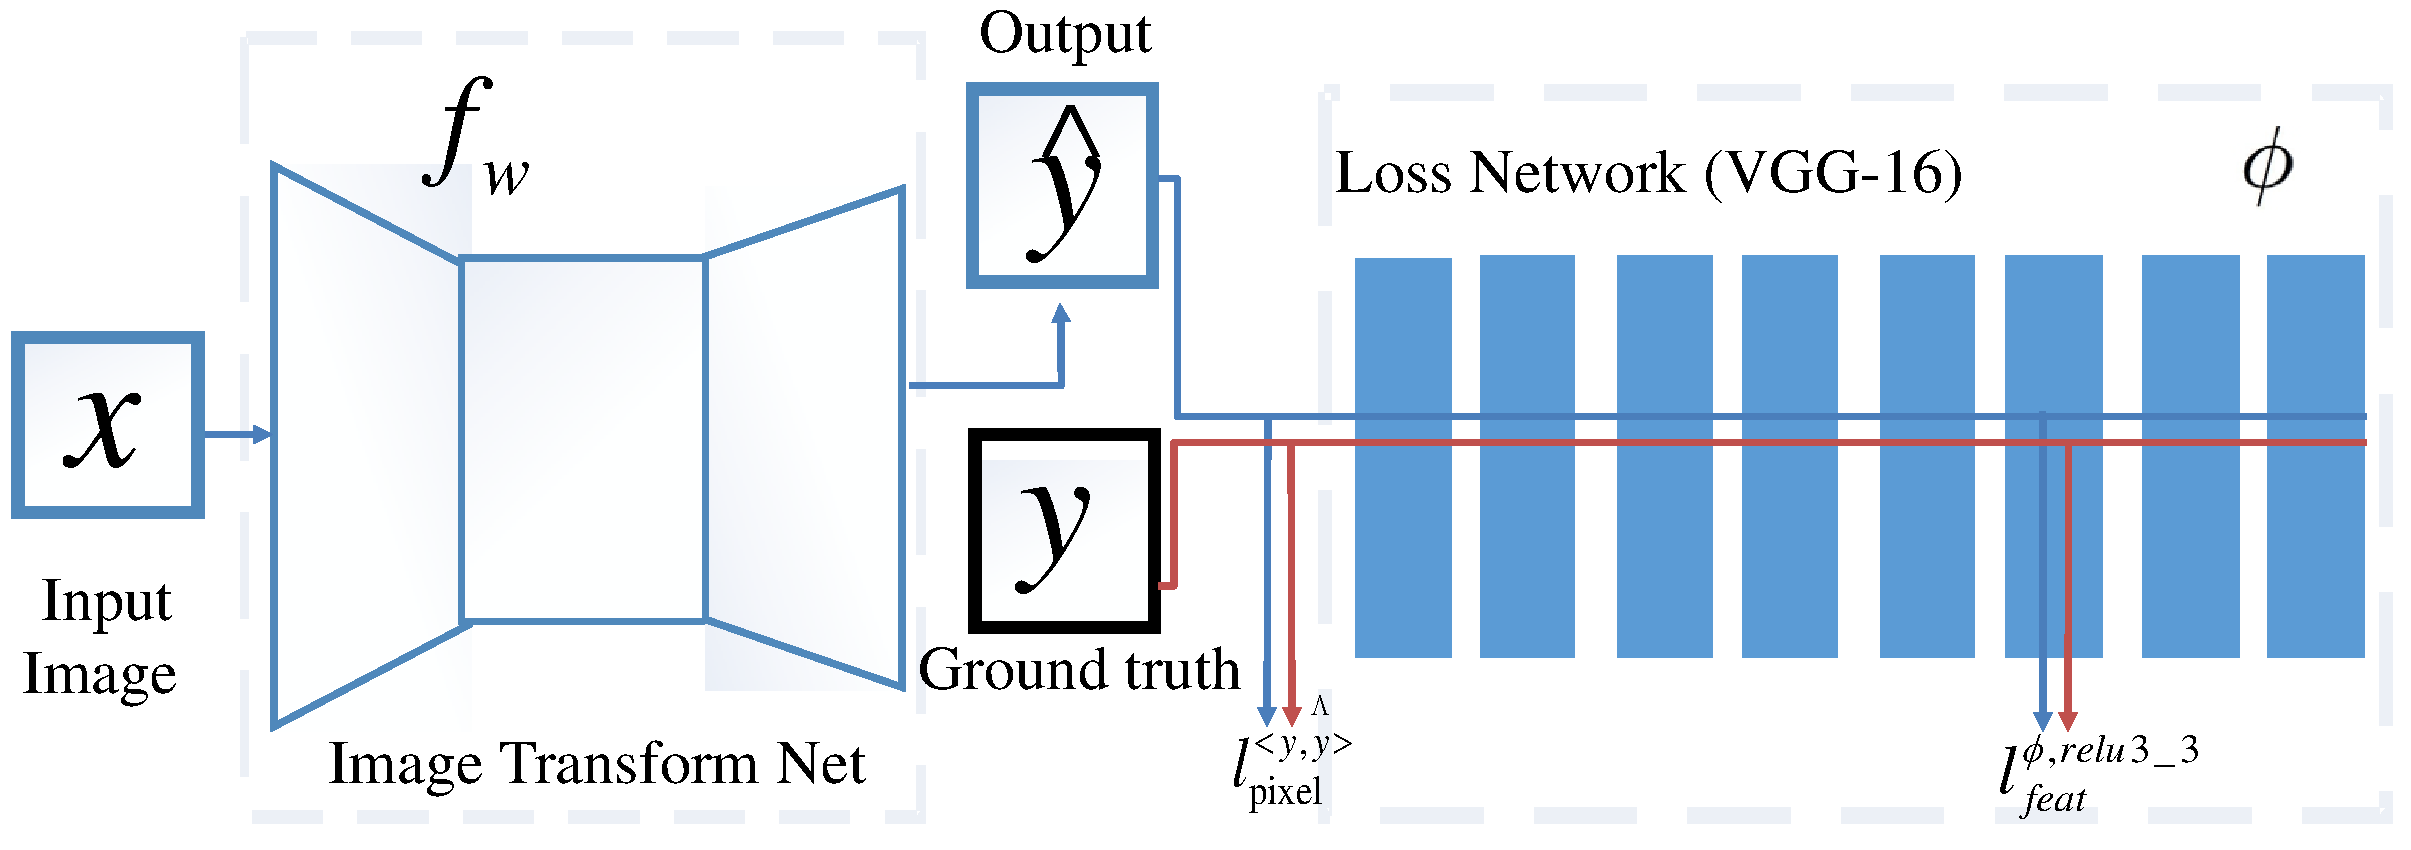
\includegraphics[width=0.58\textwidth]{ch06_01}
\caption{The overall architecture of our proposed network.
    The image transformation network contains layers of convolution (encoder)  and deconvolution (decoder). We use a loss network pretrained for image classification to define perceptual loss functions that measure perceptual differences in output and ground truth label. The loss network remains fixed during the training process.}
\label{fig:ch06_01}
\vspace{-10mm}
\end{figure*}
 

The proposed framework mainly contains a chain of convolution layers and deconvolution layers, as shown in Figure \ref{fig:ch06_01}. There consists of two components: an \emph{image transformation network} $f_W$ and a \emph{loss network} $\phi$ that is used to define several \emph{loss functions} $\ell_1,\ldots,\ell_k$. Aim at learning the deep residual convolutional neural network parameterized by weights $W$; it transforms input images $x$ into output images $f_W$ via the mapping $\hat y = f_W(x)$. 
Each loss function computes a scalar value $\ell_i(\hat y, y_i)$ measuring the difference between the output image $\hat y$ and a \emph{target image} $y_i$. Learning objective is trained using stochastic gradient descent to minimize a weighted combination of loss functions:

\begin{equation}
   W^* = \arg\min_W E_{x, \{y_i\}}\begin{bmatrix}
\sum_{i=1} \lambda_i \ell_i(f_W(x), y_i)
\end{bmatrix}
\end{equation}

From this formulation, we can see that the task here is to find a mapping function $f_W$ that best approximates the image transformation. Meanwhile we also want the $f_W(y_i)$ approxiamates the image $y_i$, so we now treat the image denoising problems in a unified framework by choosing appropriate weights $W$ with different situations. The loss network $\phi$ is used to define a \emph{feature space loss} $\ell_{feat}^\phi$ and a \emph{per-pixel loss} $\ell_{mse}$ that measure differences in feature and image space. For image denoinsing, the input image $x$ is a noisy input, the ground-truth image $y$ is also input image and target image. 
\begin{figure}[t]
\centering
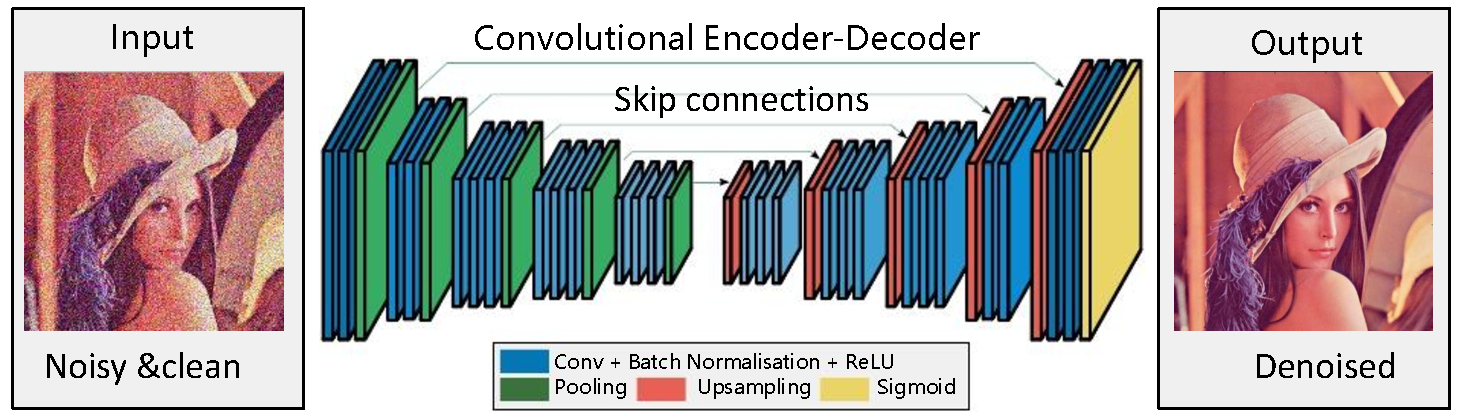
\includegraphics[width=0.58\textwidth]{ch06_02}
\caption{ The architecture of RED-NET and our image transformation network DeNET can be viewed as the RED-NET inserted some residual block. }
\label{fig:ch06_02}
\vspace{-6mm}
\end{figure} 
\subsection{Encoder-decoder Architectures}
 The framework is fully Encoder-decoder convolution model. Combining layers of encoder and decoder ~\cite{DBLP:conf/iccv/NohHH15,hong2015decoupled,DBLP:conf/cvpr/LongSD15,DBLP:journals/pami/DongLHT16,Mao2016} have been proposed for unsupervised and supervised deep learning. 

Our image transformation networks roughly follow the architectural guidelines set forth by~\cite{Mao2016}. They propose RED-NET for image denoising, the network as shown in Figure \ref{fig2}. Base on the architecture , The batch normalization~\cite{Ioffe2015Batch}and ReLU nonlinearities layers are added after convolution. And insert some residual blocks~\cite{HeZRS15} into the network.  The output layer, which  uses a sigmoid function to ensure that the output image has pixels in the range [0, 1]. But we do not use any pooling layers, instead using strided and fractionally strided convolutions for downsampling and upsampling. Other than the first and last layers which use 9$\times$9 kernels, all convolution layers use 3$\times$3 kernels. Since the image transformation networks are fully-convolutional, at test-time they can be applied to images of any size.

The difference between RED-NET and ours DeNET is that our network  insert some residual block and introduce residual connection. The noise is eliminated step by step after each layer. During this process, the details of the image content can be compensate by the perceptual loss function.  The specific configurations of the two networks are described in Table \ref{table1}.

Two learning strategy is applied to inner blocks of the encoding-decoding network to make training more effective. Skip connections are passed every two convolutional layers to their mirrored deconvolutional layers. He et.al~\cite{HeZRS15} use residual connections to train very deep networks for image classification. They argue that residual connections make  the network to learn the identify function easily; this is an appealing property for image transformation networks, since in most cases the output image should share structure with the input image. The body of our network thus consists of several residual blocks, each of which contains two 3$\times$3 convolution layers.
\begin{table}
\vspace{-4mm}
\centering
\caption{Configurations of the DeNET-R and RED-NET networks. "conv3" and "deconv3" stand for convolution and deconvolution kernels of size $3\times3$. 32,128 and  512 is the number of feature maps after each convolution and deconvolution. "$c$" is the number of channels of input and output image. i.e., $c = 3$. }
\begin{tabular}{l | l }\hline
DeNET-R                   &RED-NET                \\ \hline
(conv9-32)$\times$6             &(conv3-128)$\times$6       \\ \hline
(conv3-64)$\times$6             &(conv3-256)$\times$6       \\ \hline
(conv3-128)$\times$3             &(conv3-512)$\times$3       \\ \hline
Residual block$\times$5 &                           \\ \hline
(deconv3-64)$\times$2           &(deconv3-512)$\times$2       \\ \hline
(deconv3-32)$\times$6           &(deconv3-512)$\times$6       \\ \hline
(deconv9-3) $\times$6           &(deconv3-512)$\times$6       \\ \hline
(deconv3-$c$)           &(deconv3-$c$)                \\ \hline
\end{tabular}
\label{table1}
%\vspace{-15mm}
\end{table}
\subsection{Per-pixel Loss Functions}
The \emph{pixel loss} is the (normalized) Euclidean distance between the output image
$\hat y$ and the target $y$. If both have shape $C\times H\times W$, then the pixel Euclidean loss is
defined as Mean Squared Error(MSE): 
 \begin{equation}
   \ell_2(\hat y, y) = \frac{1}{CHW}\|\hat y - y\|_2^2
  \end{equation}
This loss function can introduce splotchy artifacts, So we also examine the \lone-norm loss. The two losses weigh errors differently:\lone does not over-penalize larger errors and consequently, they may have different convergence properties.Computing the \lone loss is straightforward:
\begin{equation}
\ell_1(\hat y, y) = \frac{1}{CHW}| \hat y - y|
\end{equation}
The derivatives for the back-propagation are also simple,  for each pixel $p$ in the whole image,
\begin{equation}
\partial \ell_1/\partial p  = sign\left(\hat y(p) - y(p)\right)
\end{equation}
Note that, although $L_{\ell_1}$ is computed on the whole image, the derivatives are back-propagated for each pixel in the image. The network trained with \lone provides a significant improvement for several of the issues discussed above.
\subsection{Perceptual Loss Functions}

We define \emph{perceptual loss functions} that measure perceptual and semantic differences between images,other than the hand design SSIM loss in~\cite{Zhao2015}. They make use of a \emph{loss network} $\phi$ pretrained
for image classification. In all our experiments $\phi$ is the 
16-layer VGG network~\cite{Simonyan14c} pretrained on the ImageNet dataset~\cite{Deng2009ImageNet}.
Rather than encouraging the pixels of the output image $\hat y=f_W(x)$ to exactly match
the pixels of the target image $y$, we instead encourage them to have similar feature
representations as computed by the loss network $\phi$. Let $\phi_j(x)$ be the activations
of the $j$th layer of the network $\phi$ when processing the image $x$; if $j$ is a
convolutional layer then $\phi_j(x)$ will be a feature map of shape
$C_j \times H_j \times W_j$. The \emph{feature feat loss} is
the (squared, normalized) Euclidean distance between feature representations:
\begin{equation}
  \ell_{feat}^{\phi,j}(\hat y, y) = 
  \frac1{C_jH_jW_j}\|\phi_j(\hat y) - \phi_j(y)\|_2^2
\end{equation}

The Euclidean distance also can be alternated by $\ell_{1}$-norm distance. As demonstrated in \cite{Mahendran2015}, finding an image $\hat y$ that minimizes the feature
feat loss for early layers tends to produce images that are visually indistinguishable from $y$. 
Using a feature feat loss for training our image transformation networks encourages
the output image $\hat y$ to be perceptually similar to the target image $y$, but does not force them to match exactly.
To encourage spatial smoothness in the output image $\hat y$, we
follow prior work on feature inversion \cite{Mahendran2015} and make use of \emph{total variation regularizer} $\ell_{TV}(\hat y)$.
 
\section{实验结果分析和讨论}
\label{sec:experiments-results}

In this section, We provide an analysis on our experiments setting with fully encoder-decoder convolutional neural network. Then evaluate denoising performance of our models under some different loss function setting. At the end we explore how to make one neural network handle different levels of noise.
\subsection{Analysis On Model Details}
\begin{table}[b]\label{tab:Denoising-results}  
\vspace{-4mm} 
   \centering{
   \caption{Quantitative single-level image denoising results 
     on the Set14; we report average PSNR and SSIM on each dataset.
     each $\sigma$ value we train identical networks, one with a 
     per-pixel loss $\ell_{1}$,$\ell_{2}$ and another with a feature feat loss $\ell_{feat}$.$\ell_{mix}$ is combine with $\ell_{1}$and $\ell_{feat}$.Best results are shown in bold.   
   }
   \scalebox{0.80}{
     \begin{tabular}{|c|c|c|c|c|c|c|}
       \hline
        \multirow{2}{*}{Sigma} & Noisy & RED-NET~\cite{Mao2016} & Ours ($\ell_{2})$ & Ours ($\ell_{1}$)& Ours ($\ell_{feat}$) & Ours ($\ell_{mix}$)\\
   & PSNR / SSIM & PSNR / SSIM & PSNR / SSIM & PSNR / SSIM & PSNR / SSIM & PSNR / SSIM\\
   \hline
    \multirow{1}{*}{$\sigma=10$} & 28.16 / 0.7041 & \textbf{34.81} / \textbf{0.9402}
           & 34.35 / 0.8912 & 33.40 / 0.8930& 31.05 / 0.7680& 33.16 / 0.7680  \\
          % \hline 
    \multirow{1}{*}{$\sigma=30$} & 18.88 / 0.3389 & 29.17 / 0.8423
           & 28.73 / 0.8205 & 29.76 / 0.8591& 26.70 / 0.6845& \textbf{30.15} / \textbf{0.8681}  \\
          % \hline
    \multirow{1}{*}{$\sigma=50$} & 14.79 / 0.2038 & 26.81 / 0.7733
           & 26.40 / 0.8205 & 26.79 / \textbf{0.8325}& 25.69 / 0.6411& \textbf{27.09} / 0.8312  \\
          % \hline
    \multirow{1}{*}{$\sigma=70$} & 12.43 / 0.1391 & 25.31 / 0.7206
           & 25.39 / 0.7105 & 26.13 / \textbf{0.7250}& 17.89 / 0.6650& \textbf{26.20} / 0.7180  \\
    \multirow{1}{*}{$\sigma=100$} & 10.26 / 0.0901 &  -
           & 18.40 / 0.4215 & 20.19 / 0.4680& 17.31 / 0.3640& \textbf{19.16} / \textbf{0.4695}  \\
           \hline
        
\end{tabular} 
}}  
\vspace{-4mm}
\end{table}
We train models to perform single and multi level of standard deviation $\sigma$ by minimizing some loss function: $\ell_{2}$-Mean Squared Error(MSE) loss,$\ell_{1}$-norm loss and feature feat loss at layer \verb.relu1_1. from the VGG-16 network $\phi$. We train image size with $256\times256$ from the training set, and prepare noisy inputs by add a Gaussian kernel of width $\sigma$. We train with a batch size of 10 using Adam~\cite{Kingma2014Adam} with a learning rate of $1\times10^{-3}$ without weight decay or dropout. 

Denoising experiments are performed on the standard 14 common benchmark images Set14. As a common experimental setting in the literature, additive Gaussian noises with zero mean and standard deviation $\sigma$ are added to the test image to test the performance of denoising methods. We report PSNR and SSIM~\cite{Wang2004}, computing both on the three channel color image, following~\cite{Mao2016,Zhao2015}.

As a baseline model we use RED-NET~\cite{Mao2016} for its state-of-the-art performance. Its is a fully convolutional network with convolutonal and deconvolutonal layers trained to minimize per-pixel loss. To account for differences between RED-NET and our model in data, training, and architecture, we train image transformation networks for the same standard deviation $\sigma$ using $\ell_{2}$; these networks use identical data, architecture, and training as the networks trained to minimize other loss function. We train denoising networks with the per-pixel loss typically used~\cite{Mao2016,Zhao2015}, also with a feature feat loss (see Section~\ref{sec:method}) to allow transfer of semantic knowledge from the pretrained loss network to the denoising network as supervised signal guided denoising.


\begin{figure}[t]
\centering
  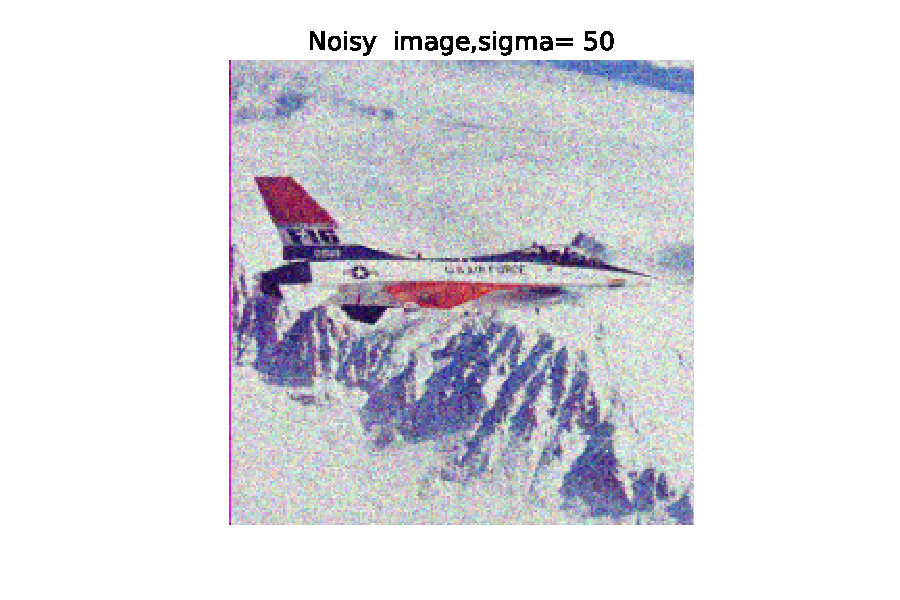
\includegraphics[width=0.19\textwidth]{figs/loss/noisy.pdf}
  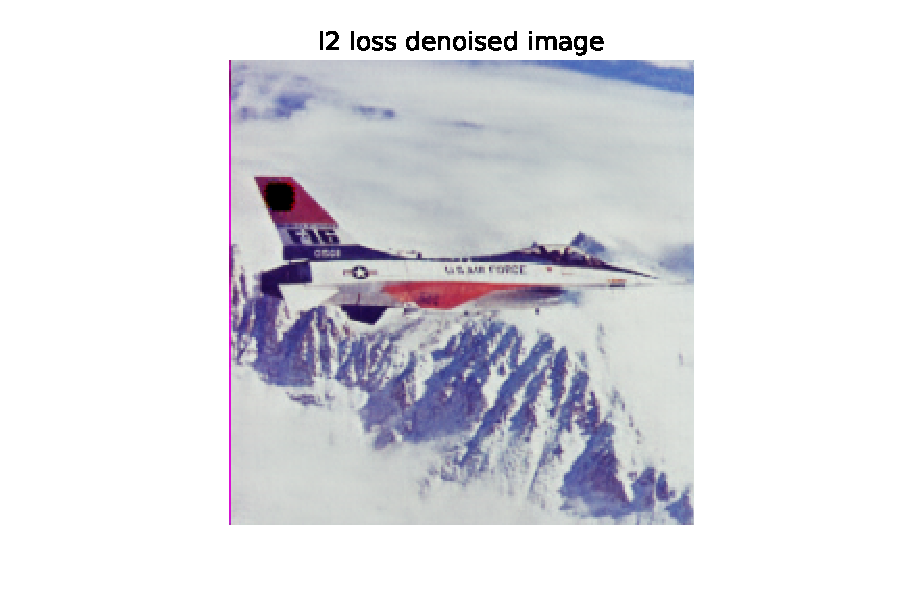
\includegraphics[width=0.19\textwidth]{figs/loss/l2.pdf}
  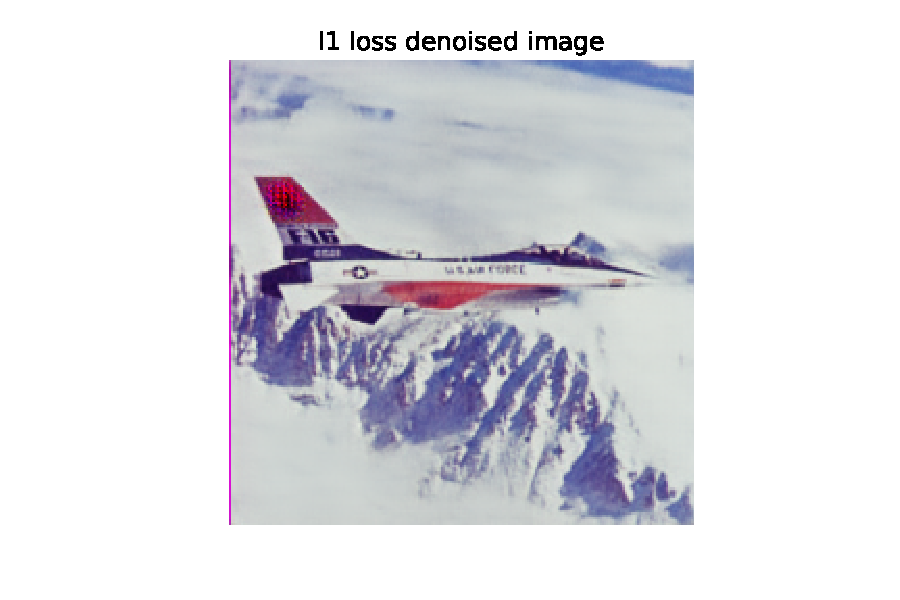
\includegraphics[width=0.19\textwidth]{figs/loss/l1.pdf}
  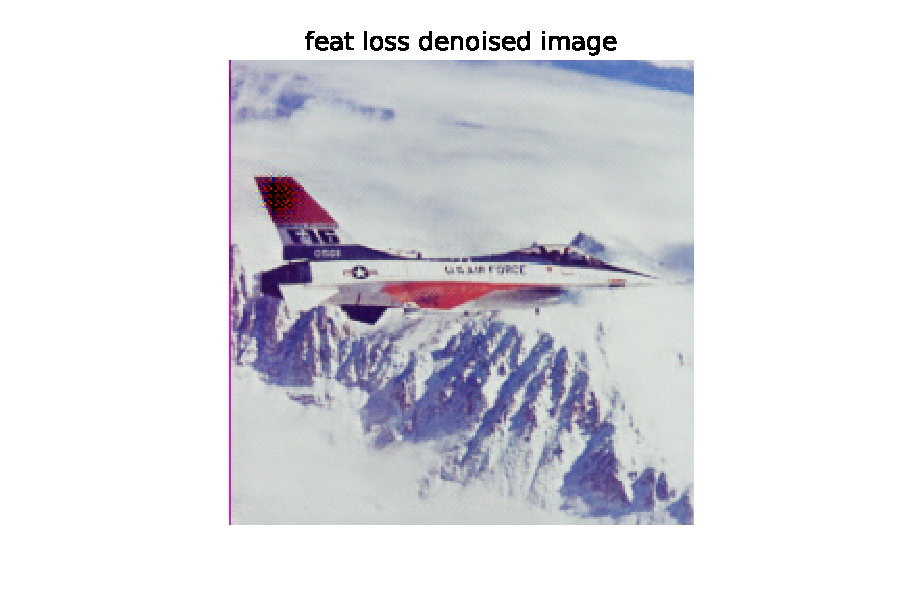
\includegraphics[width=0.19\textwidth]{figs/loss/feat.pdf}
  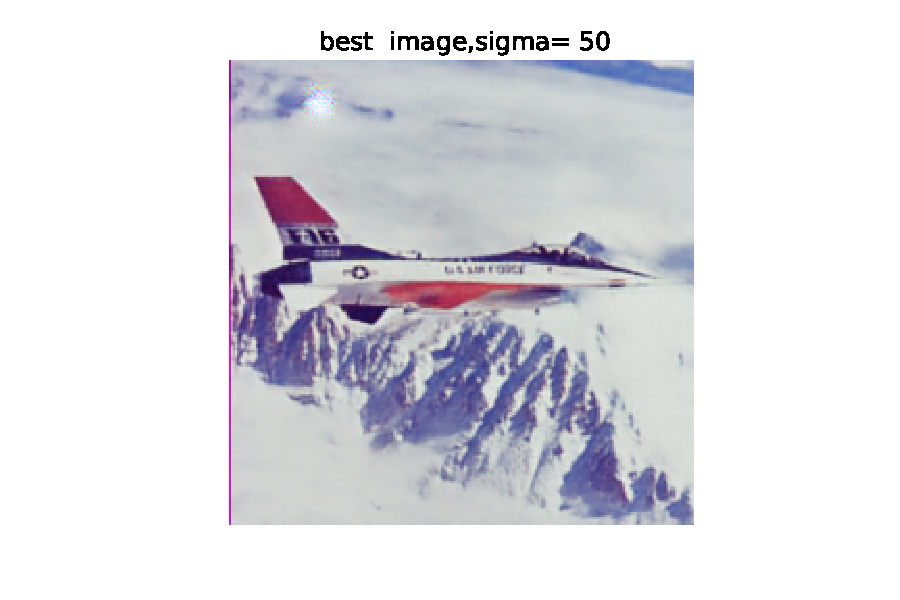
\includegraphics[width=0.19\textwidth]{figs/loss/mix.pdf}  \\{}
  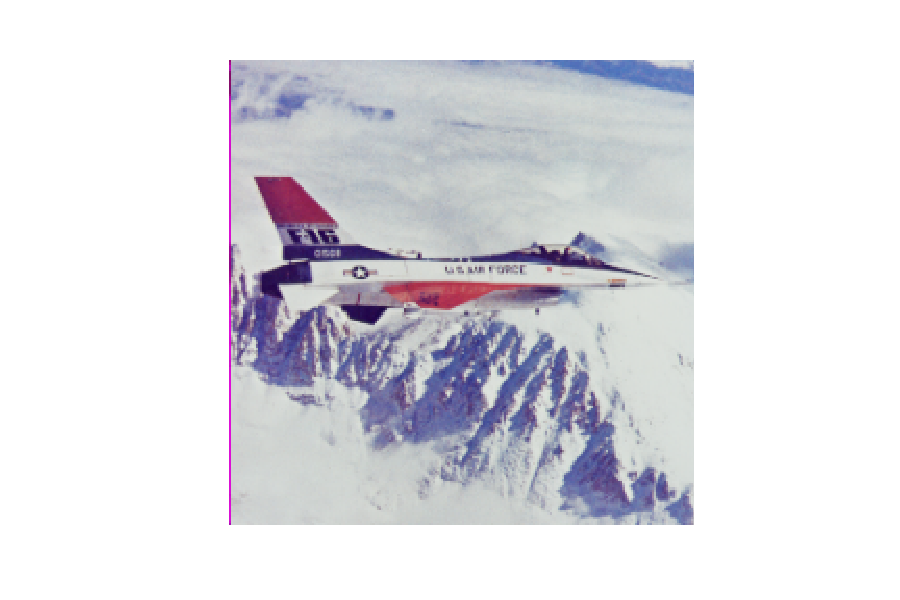
\includegraphics[trim={15pt 60pt 15pt 62pt},width=0.19\textwidth,clip]{figs/loss/orign.pdf}
  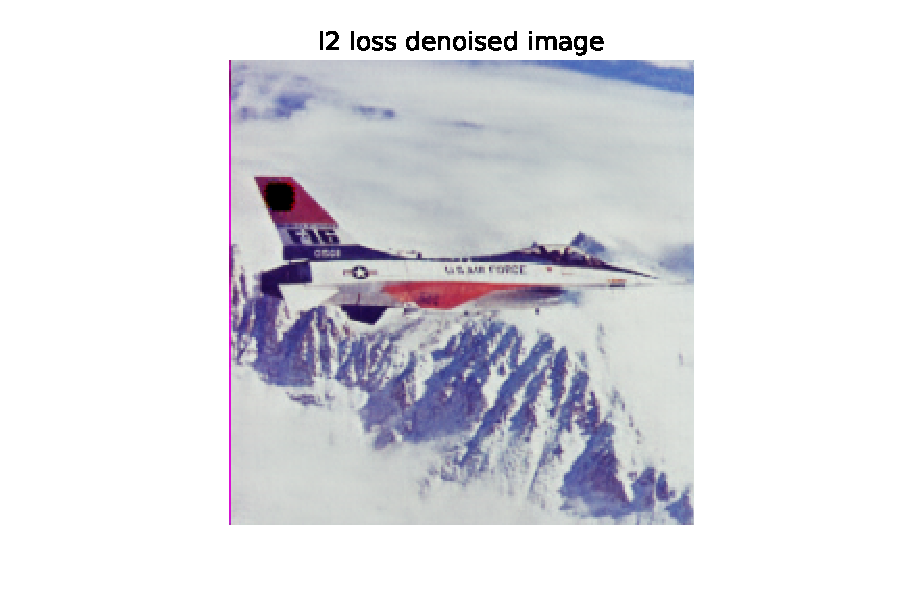
\includegraphics[trim={15pt 60pt 15pt 75pt},width=0.19\textwidth,clip]{figs/loss/l2.pdf}
  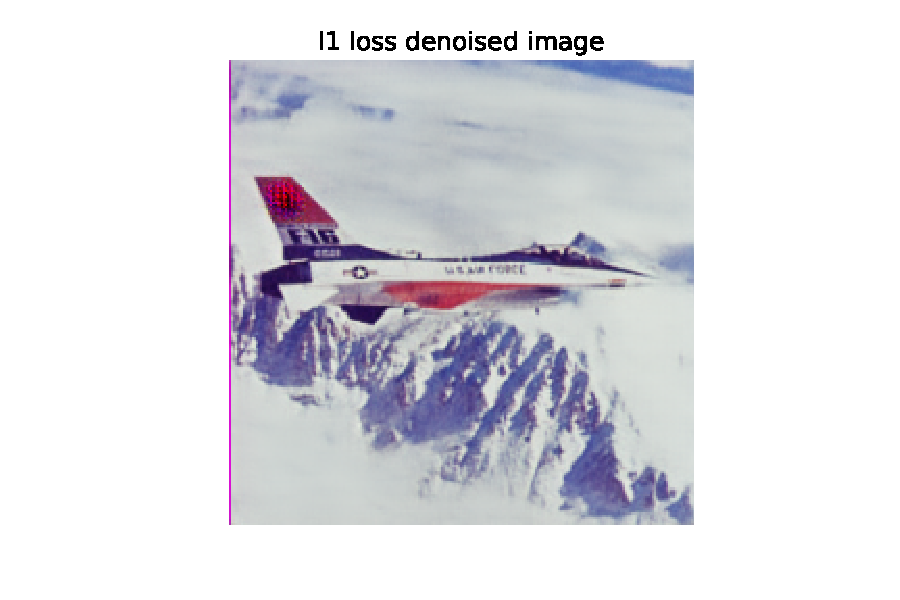
\includegraphics[trim={15pt 60pt 15pt 75pt},width=0.19\textwidth,clip]{figs/loss/l1.pdf}
  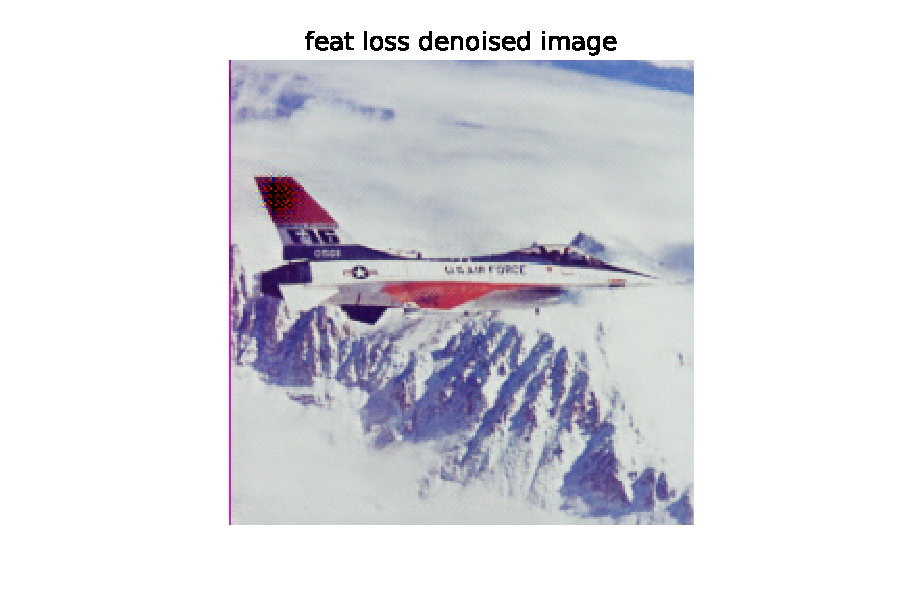
\includegraphics[trim={15pt 60pt 15pt 75pt},width=0.19\textwidth,clip]{figs/loss/feat.pdf}
  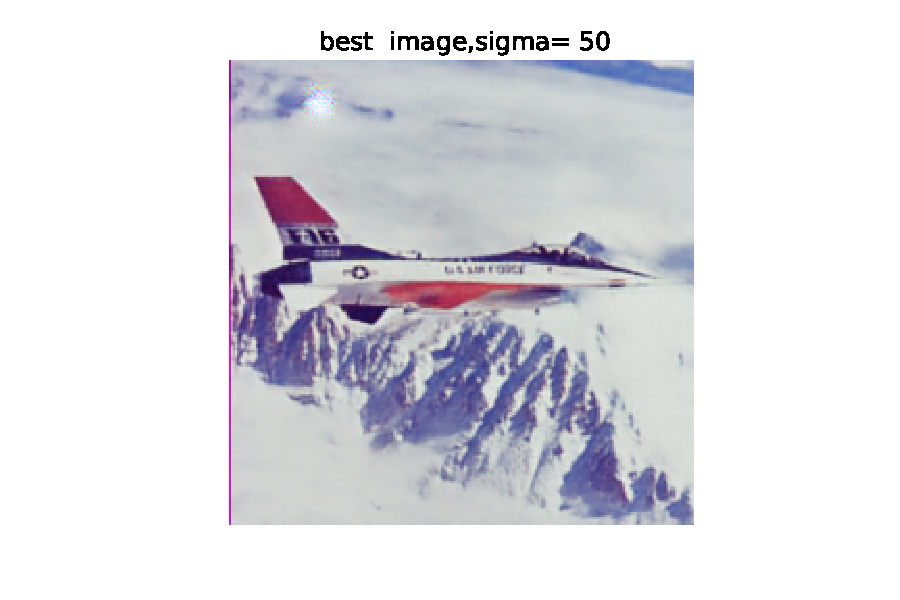
\includegraphics[trim={15pt 60pt 15pt 75pt},width=0.19\textwidth,clip]{figs/loss/mix.pdf} \\
   \begin{minipage}{0.19\textwidth}
        \centering \textbf{Ground Truth} \\ PSNR / SSIM
   \end{minipage}
   \begin{minipage}{0.19\textwidth}
     \centering \textbf{Ours}($\ell_{2}$) \\ 29.11 / 0.8833
   \end{minipage}
   \begin{minipage}{0.19\textwidth}
     \centering \textbf{Ours} ($\ell_{1}$) \\ 29.27 / 0.8841
   \end{minipage}
   \begin{minipage}{0.19\textwidth}
     \centering \textbf{Ours} ($\ell_{feat}$) \\  19.61 / 0.6560
   \end{minipage}
   \begin{minipage}{0.19\textwidth}
     \centering \textbf{Ours} ($\ell_{mix}$) \\  29.31 / 0.8946
   \end{minipage} \\
  \caption{Denoising results with different loss type on an image from the
    Set14 dataset. We report PSNR / SSIM for the  F16-plane image as a example. 
  }
  \vspace{-4mm}
  \label{fig:l1-l2-feat-results}
\end{figure}

First of all, Compared to the per-pixel loss $\ell_{1}$ and $\ell_{2}$ result, $\ell_{1}$ does a better good job at denoising performance and meanwhile restore sharp edges and fine details. As show in Figure~\ref{fig:l1-l2-feat-results}
the wing in the $\ell_{2}$ image and the red color block elements of the body in the $\ell_{2}$ image.This is because $\ell_{2}$ penalizes larger errors, but is more tolerant to small errors, regardless of the underlying structure in the image; The conclusion is consistent with the literature~\cite{Zhao2015}.

Moreover, Results for $\ell_{feat}$ are Show in Figure~\ref{fig:l1-l2-feat-results} when only with the feature feat loss gives rise to a slight cross-hatch pattern visible under magnification, which harms its PSNR and SSIM compared to baseline methods. Again we see that our $\ell_{feat}$ model does a good job at edges and fine details compared to other models, such as the wing. The $\ell_{feat}$ model does not sharpen edges indiscriminately; compared to the $\ell_{pixel}$ model, the $\ell_{feat}$ model sharpens the boundary edges of the wing and rider but the background mountain remain diffuse, suggesting that the $\ell_{feat}$ model may be more aware of image semantics.

Since our $\ell_{pixel}$ and our $\ell_{feat}$ models share the same architecture, data, and training procedure, all differences between them are due to the difference between the $\ell_{pixel}$ and $\ell_{feat}$ losses. The $\ell_{pixel}$ loss gives fewer visual artifacts and higher PSNR values but the $\ell_{feat}$ loss does a better job at reconstructing fine details, leading to pleasing visual results.

Last, we can observe that a single model can work across all levels of Gaussian noise,thereby allowing to reduce significantly the training time for a general-purpose neural network powered denoising algorithm. The reason for this may be that the learned image transformation function can model the Gaussian-like distribute from any levels and other types. Interesting is that shown in Figure~\ref{fig:other-type-results},
even for other type of noise ,such as speckle noise,poission-distributed noise,salt noise or pepper noise, which the model trained for Gaussian noise have ability for image denoise.
   \begin{figure}[t]
 \centering
   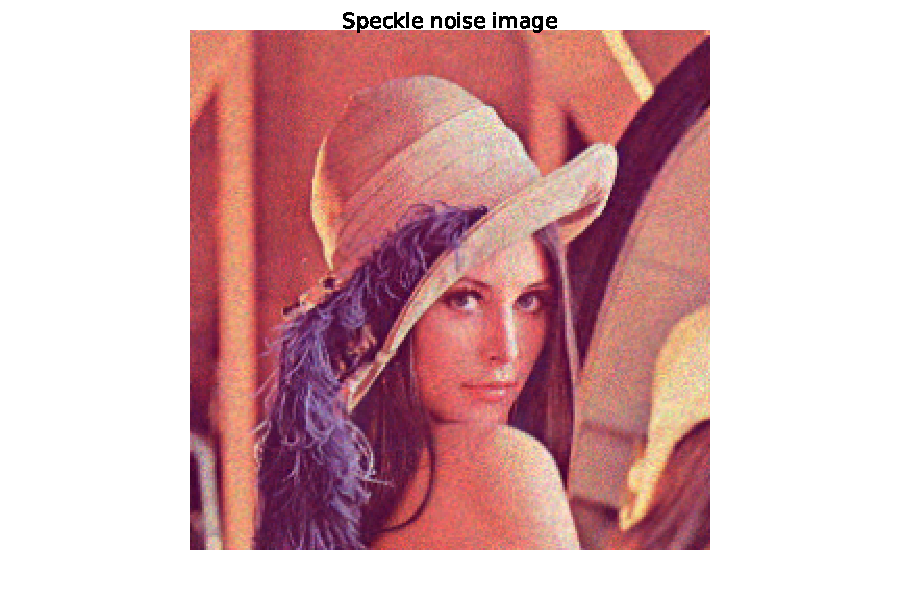
\includegraphics[width=0.24\textwidth]{figs/speckle}
  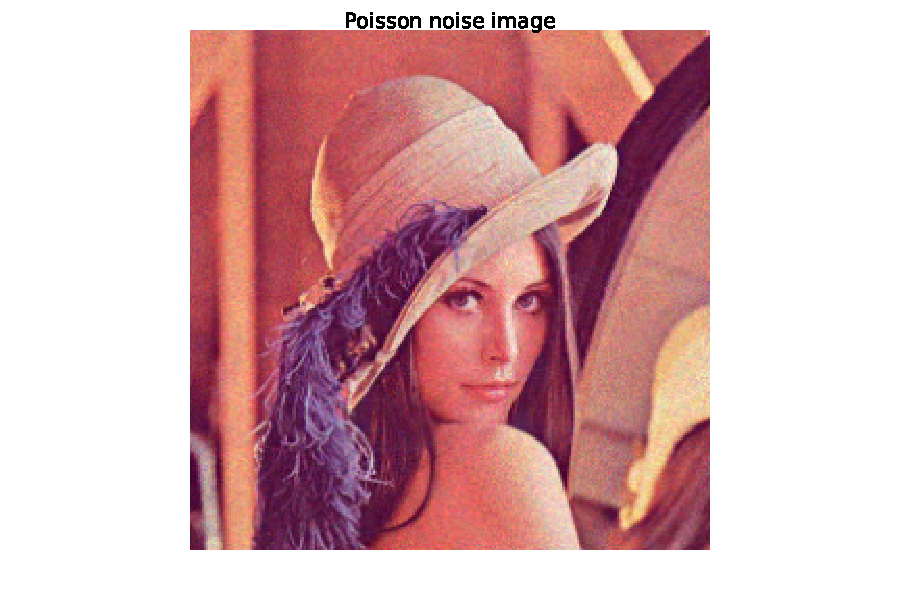
\includegraphics[width=0.24\textwidth]{figs/poisson}
  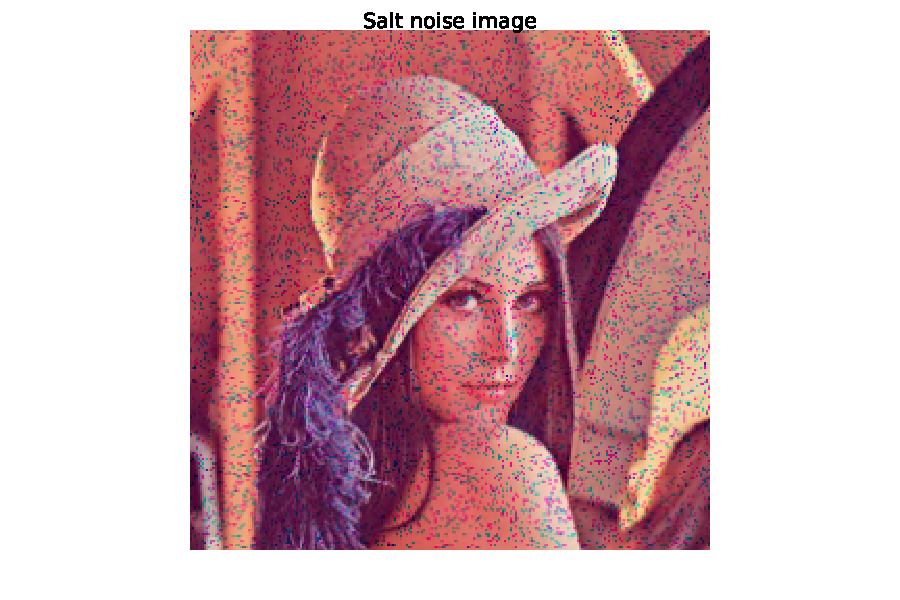
\includegraphics[width=0.24\textwidth]{figs/salt}
  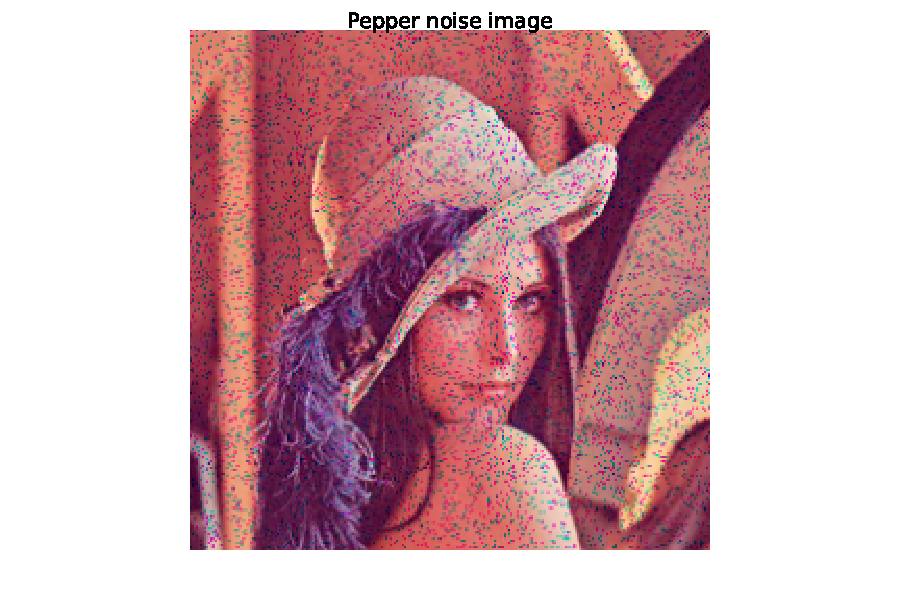
\includegraphics[width=0.24\textwidth]{figs/pepper} \\{}
  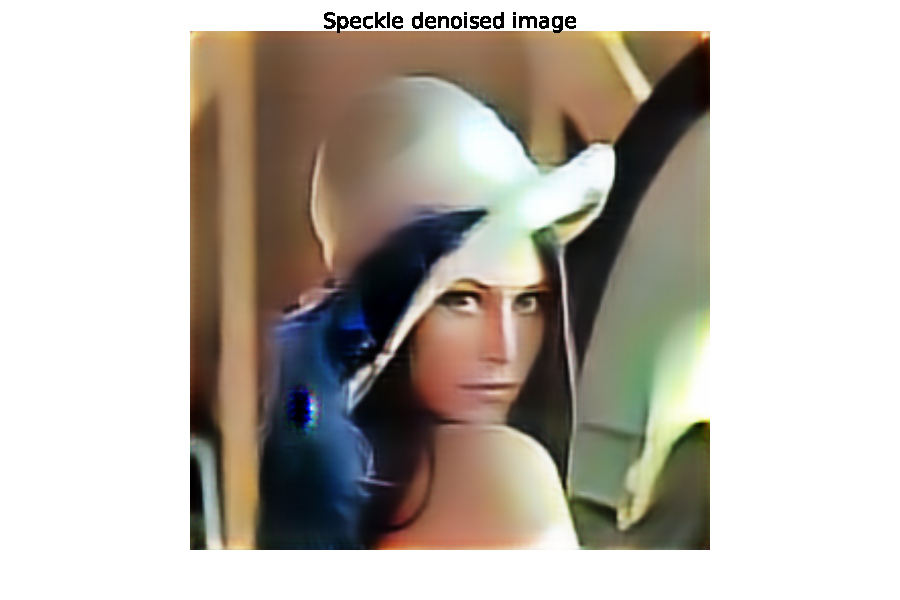
\includegraphics[trim={160pt 30pt 150pt 200pt},width=0.24\textwidth,clip]{figs/speckle_denoised}
  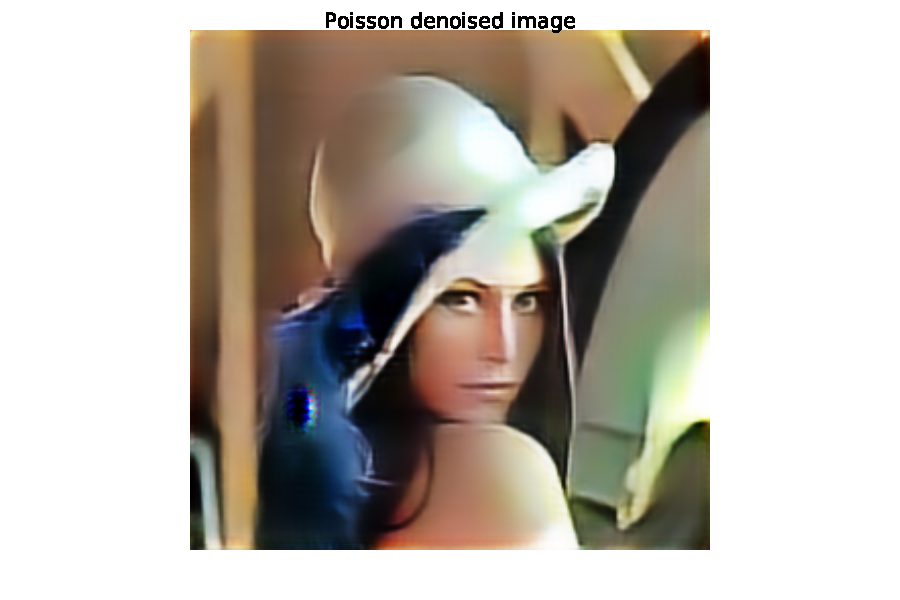
\includegraphics[trim={160pt 30pt 150pt 200pt},width=0.24\textwidth,clip]{figs/poisson_denoised}
  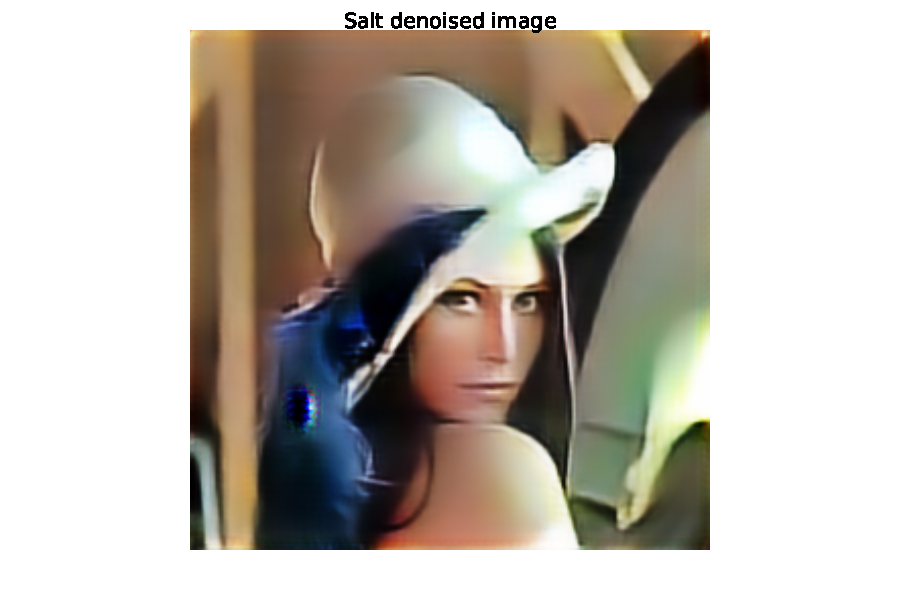
\includegraphics[trim={160pt 30pt 150pt 200pt},width=0.24\textwidth,clip]{figs/salt_denoised}
  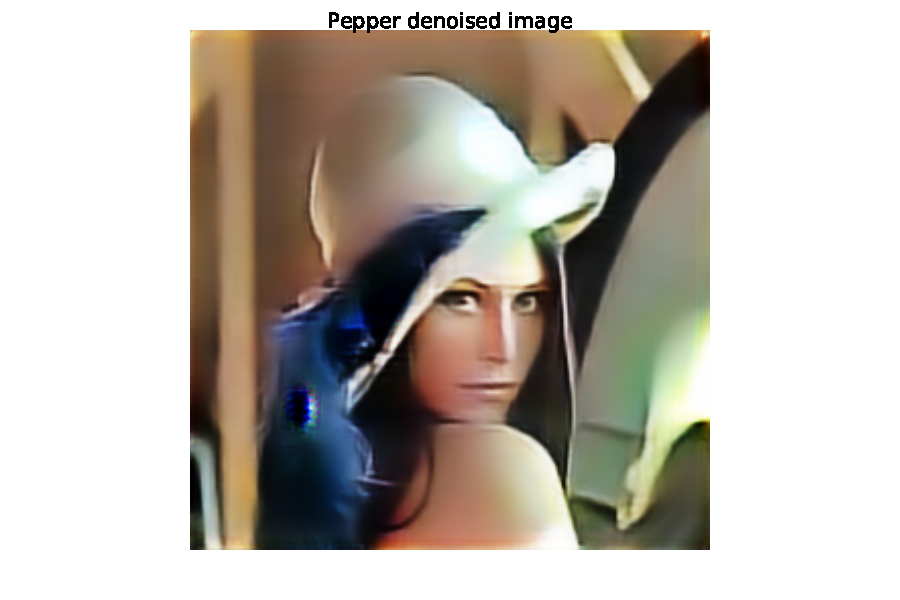
\includegraphics[trim={160pt 30pt 150pt 200pt},width=0.24\textwidth,clip]{figs/pepper_denoised} \\
    
   \caption{Comparison denoising performance of four other noise types ,which  transformation networks trained only with Gaussian noise. \textbf{Up:} The four types noise image:Speckle noise,Poisson distributed noise,Salt noise,Pepper noise. \textbf{Down:} Denoising sub-outputs from corresponding noise type.
   }
   \vspace{-4mm}
   \label{fig:other-type-results}
 \end{figure}
 

\section{小结与讨论}

